\hypertarget{xmlrpc_8inc}{
\section{include/xmlrpc.inc File Reference}
\label{xmlrpc_8inc}\index{include/xmlrpc.inc@{include/xmlrpc.inc}}
}
XML-RPC Library. 

\subsection*{Classes}
\begin{CompactItemize}
\item 
class \hyperlink{classXML}{XML}
\end{CompactItemize}
\subsection*{Functions}
\begin{CompactItemize}
\item 
\& \hyperlink{xmlrpc_8inc_a1e9b05a06f28fabb86c10129f5890ef}{XML\_\-serialize} (\&\$data, \$level=0, \$prior\_\-key=NULL)
\item 
\& \hyperlink{xmlrpc_8inc_ef8f3de498a12b230d049cdee6a25145}{XML\_\-unserialize} (\&\$xml)
\item 
\& \hyperlink{xmlrpc_8inc_708b2136ca600664d2207a511b3cf3f8}{XMLRPC\_\-parse} (\&\$request)
\item 
\& \hyperlink{xmlrpc_8inc_c13be54b26e0803d8745e4f019dcfd8a}{XMLRPC\_\-prepare} (\$data, \$type=NULL)
\item 
\& \hyperlink{xmlrpc_8inc_d936fe41ae9c3e0b90bd72ffe82a2969}{XMLRPC\_\-adjustValue} (\&\$current\_\-node)
\item 
\hyperlink{xmlrpc_8inc_ce4ea8e1274ca2ee3f51ec5a724f00f3}{XMLRPC\_\-getParams} (\$request)
\item 
\hyperlink{xmlrpc_8inc_70efa062e92a380196ed8053850c0906}{XMLRPC\_\-getMethodName} (\$methodCall)
\item 
\hyperlink{xmlrpc_8inc_3a98b6984b8ca01752d1aa9a267526a3}{XMLRPC\_\-request} (\$site, \$location, \$methodName, \$params=NULL, \$user\_\-agent=NULL)
\item 
\hyperlink{xmlrpc_8inc_c736d378caaccdd0726ea1080d1f526f}{XMLRPC\_\-response} (\$return\_\-value, \$server=NULL)
\item 
\hyperlink{xmlrpc_8inc_0cdc54b1376ccbbe412175c9819a95ac}{XMLRPC\_\-error} (\$faultCode, \$faultString, \$server=NULL)
\item 
\hyperlink{xmlrpc_8inc_4485d809c5d598949d9cfaca42bddf37}{XMLRPC\_\-convert\_\-timestamp\_\-to\_\-iso8601} (\$timestamp)
\item 
\hyperlink{xmlrpc_8inc_1d9c2ef61c9f1fd2723d06d1364ef845}{XMLRPC\_\-convert\_\-iso8601\_\-to\_\-timestamp} (\$iso8601)
\item 
\hyperlink{xmlrpc_8inc_88839ba2c5c835c99f55578c65faa401}{count\_\-numeric\_\-items} (\&\$array)
\item 
\hyperlink{xmlrpc_8inc_e2d2e97a8c1c560f5e96d58d60a02874}{XMLRPC\_\-debug} (\$function\_\-name, \$debug\_\-message)
\item 
\hyperlink{xmlrpc_8inc_8467f85edd385ddf2506b1bd5065a6d7}{XMLRPC\_\-debug\_\-print} ()
\item 
\hyperlink{xmlrpc_8inc_1f60d2672bcb35f5ff908f64931f8d48}{XMLRPC\_\-show} (\$data, \$func=\char`\"{}print\_\-r\char`\"{}, \$return\_\-str=false)
\end{CompactItemize}


\subsection{Detailed Description}
XML-RPC Library. 

An XML-RPC implementation by Keith Devens, version 2.5f. \href{http://www.keithdevens.com/software/xmlrpc/}{\tt http://www.keithdevens.com/software/xmlrpc/} Release history available at: \href{http://www.keithdevens.com/software/xmlrpc/history/}{\tt http://www.keithdevens.com/software/xmlrpc/history/} This code is Open Source, released under terms similar to the Artistic License. Read the license at \href{http://www.keithdevens.com/software/license/}{\tt http://www.keithdevens.com/software/license/} Note: this code requires version 4.1.0 or higher of PHP.

\begin{Desc}
\item[See also:]\href{http://keithdevens.com/software/xmlrpc}{\tt http://keithdevens.com/software/xmlrpc} \end{Desc}


Definition in file \hyperlink{xmlrpc_8inc-source}{xmlrpc.inc}.

\subsection{Function Documentation}
\hypertarget{xmlrpc_8inc_88839ba2c5c835c99f55578c65faa401}{
\index{xmlrpc.inc@{xmlrpc.inc}!count_numeric_items@{count\_\-numeric\_\-items}}
\index{count_numeric_items@{count\_\-numeric\_\-items}!xmlrpc.inc@{xmlrpc.inc}}
\subsubsection{\setlength{\rightskip}{0pt plus 5cm}count\_\-numeric\_\-items (\&\$ {\em array})}}
\label{xmlrpc_8inc_88839ba2c5c835c99f55578c65faa401}




Definition at line 465 of file xmlrpc.inc.

Referenced by XML::open(), and XMLRPC\_\-prepare().

\begin{Code}\begin{verbatim}465                                      {
466   return is_array($array) ? count(array_filter(array_keys($array), 'is_numeric')) : 0;
467 }
\end{verbatim}
\end{Code}




Here is the caller graph for this function:\nopagebreak
\begin{figure}[H]
\begin{center}
\leavevmode
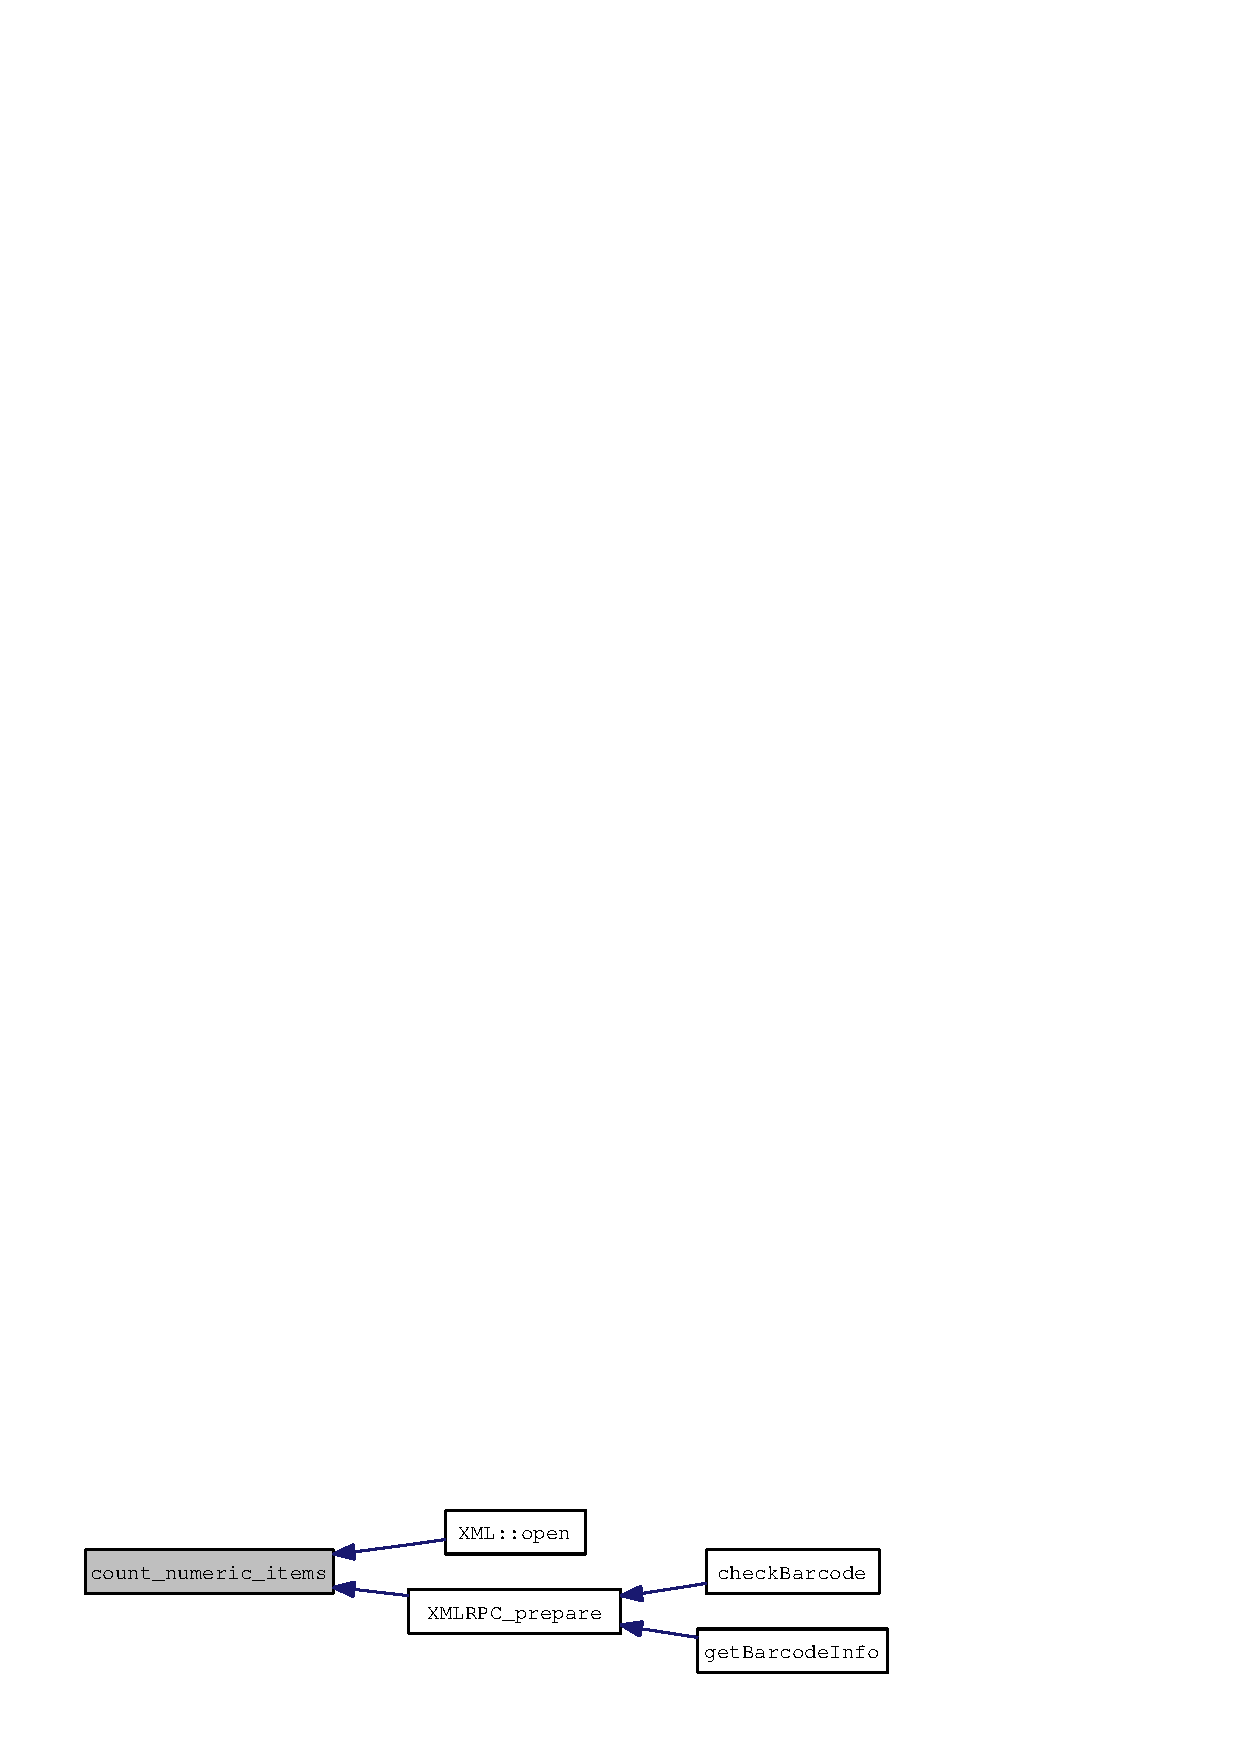
\includegraphics[width=215pt]{xmlrpc_8inc_88839ba2c5c835c99f55578c65faa401_icgraph}
\end{center}
\end{figure}
\hypertarget{xmlrpc_8inc_a1e9b05a06f28fabb86c10129f5890ef}{
\index{xmlrpc.inc@{xmlrpc.inc}!XML_serialize@{XML\_\-serialize}}
\index{XML_serialize@{XML\_\-serialize}!xmlrpc.inc@{xmlrpc.inc}}
\subsubsection{\setlength{\rightskip}{0pt plus 5cm}\& XML\_\-serialize (\&\$ {\em data}, \$ {\em level} = {\tt 0}, \$ {\em prior\_\-key} = {\tt NULL})}}
\label{xmlrpc_8inc_a1e9b05a06f28fabb86c10129f5890ef}




Definition at line 17 of file xmlrpc.inc.

Referenced by XMLRPC\_\-error(), XMLRPC\_\-request(), and XMLRPC\_\-response().

\begin{Code}\begin{verbatim}17                                                                {
18   #assumes a hash, keys are the variable names
19   $xml_serialized_string = "";
20   while(list($key, $value) = each($data)){
21     $inline = false;
22     $numeric_array = false;
23     $attributes = "";
24     #echo "My current key is '$key', called with prior key '$prior_key'<br>";
25     if(!strstr($key, " attr")){ #if it's not an attribute
26       if(array_key_exists("$key attr", $data)){
27         while(list($attr_name, $attr_value) = each($data["$key attr"])){
28           #echo "Found attribute $attribute_name with value $attribute_value<br>";
29           $attr_value = &htmlspecialchars($attr_value, ENT_QUOTES);
30           $attributes .= " $attr_name=\"$attr_value\"";
31         }
32       }
33 
34       if(is_numeric($key)){
35         #echo "My current key ($key) is numeric. My parent key is '$prior_key'<br>";
36         $key = $prior_key;
37       }else{
38         #you can't have numeric keys at two levels in a row, so this is ok
39         #echo "Checking to see if a numeric key exists in data.";
40         if(is_array($value) and array_key_exists(0, $value)){
41         # echo " It does! Calling myself as a result of a numeric array.<br>";
42           $numeric_array = true;
43           $xml_serialized_string .= XML_serialize($value, $level, $key);
44         }
45         #echo "<br>";
46       }
47 
48       if(!$numeric_array){
49         $xml_serialized_string .= str_repeat("\t", $level) . "<$key$attributes>";
50 
51         if(is_array($value)){
52           $xml_serialized_string .= "\r\n" . XML_serialize($value, $level+1);
53         }else{
54           $inline = true;
55           $xml_serialized_string .= htmlspecialchars($value);
56         }
57 
58         $xml_serialized_string .= (!$inline ? str_repeat("\t", $level) : "") . "</$key>\r\n";
59       }
60     }else{
61       #echo "Skipping attribute record for key $key<bR>";
62     }
63   }
64   if($level == 0){
65     $xml_serialized_string = "<?xml version=\"1.0\" ?>\r\n" . $xml_serialized_string;
66     return $xml_serialized_string;
67   }else{
68     return $xml_serialized_string;
69   }
70 }
\end{verbatim}
\end{Code}




Here is the caller graph for this function:\nopagebreak
\begin{figure}[H]
\begin{center}
\leavevmode
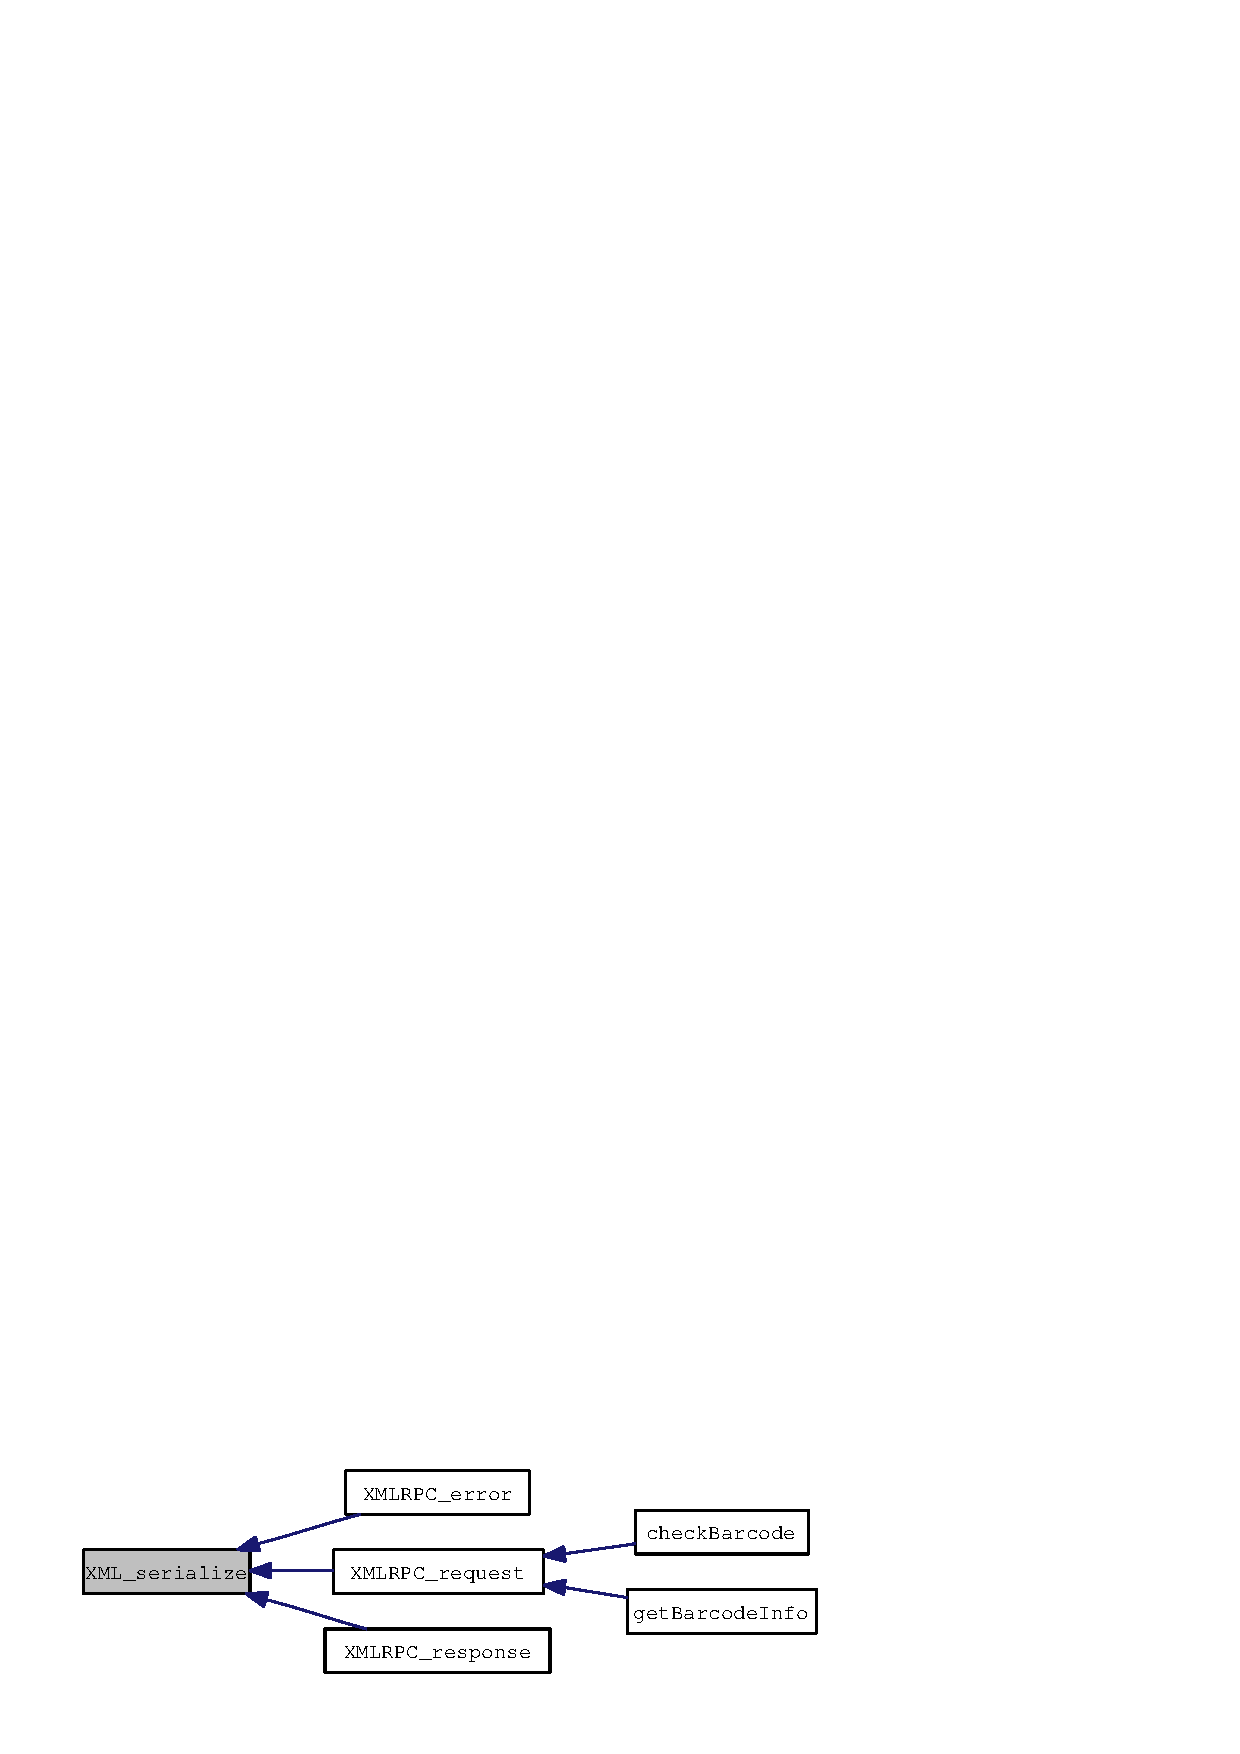
\includegraphics[width=198pt]{xmlrpc_8inc_a1e9b05a06f28fabb86c10129f5890ef_icgraph}
\end{center}
\end{figure}
\hypertarget{xmlrpc_8inc_ef8f3de498a12b230d049cdee6a25145}{
\index{xmlrpc.inc@{xmlrpc.inc}!XML_unserialize@{XML\_\-unserialize}}
\index{XML_unserialize@{XML\_\-unserialize}!xmlrpc.inc@{xmlrpc.inc}}
\subsubsection{\setlength{\rightskip}{0pt plus 5cm}\& XML\_\-unserialize (\&\$ {\em xml})}}
\label{xmlrpc_8inc_ef8f3de498a12b230d049cdee6a25145}




Definition at line 159 of file xmlrpc.inc.

Referenced by XMLRPC\_\-parse(), and XMLRPC\_\-request().

\begin{Code}\begin{verbatim}159                                  {
160   $xml_parser = new XML();
161   $data = &$xml_parser->parse(&$xml);
162   $xml_parser->destruct();
163   return $data;
164 }
\end{verbatim}
\end{Code}




Here is the caller graph for this function:\nopagebreak
\begin{figure}[H]
\begin{center}
\leavevmode
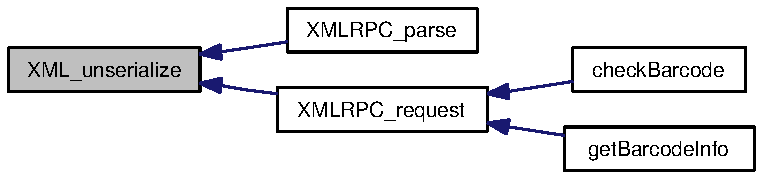
\includegraphics[width=201pt]{xmlrpc_8inc_ef8f3de498a12b230d049cdee6a25145_icgraph}
\end{center}
\end{figure}
\hypertarget{xmlrpc_8inc_d936fe41ae9c3e0b90bd72ffe82a2969}{
\index{xmlrpc.inc@{xmlrpc.inc}!XMLRPC_adjustValue@{XMLRPC\_\-adjustValue}}
\index{XMLRPC_adjustValue@{XMLRPC\_\-adjustValue}!xmlrpc.inc@{xmlrpc.inc}}
\subsubsection{\setlength{\rightskip}{0pt plus 5cm}\& XMLRPC\_\-adjustValue (\&\$ {\em current\_\-node})}}
\label{xmlrpc_8inc_d936fe41ae9c3e0b90bd72ffe82a2969}




Definition at line 237 of file xmlrpc.inc.

Referenced by XMLRPC\_\-getParams(), and XMLRPC\_\-request().

\begin{Code}\begin{verbatim}237                                              {
238   if(is_array($current_node)){
239     if(isset($current_node['array'])){
240       if(!is_array($current_node['array']['data'])){
241         #If there are no elements, return an empty array
242         return array();
243       }else{
244         #echo "Getting rid of array -> data -> value<br>\n";
245         $temp = &$current_node['array']['data']['value'];
246         if(is_array($temp) and array_key_exists(0, $temp)){
247           $count = count($temp);
248           for($n=0;$n<$count;$n++){
249             $temp2[$n] = &XMLRPC_adjustValue(&$temp[$n]);
250           }
251           $temp = &$temp2;
252         }else{
253           $temp2 = &XMLRPC_adjustValue(&$temp);
254           $temp = array(&$temp2);
255           #I do the temp assignment because it avoids copying,
256           # since I can put a reference in the array
257           #PHP's reference model is a bit silly, and I can't just say:
258           # $temp = array(&XMLRPC_adjustValue(&$temp));
259         }
260       }
261     }elseif(isset($current_node['struct'])){
262       if(!is_array($current_node['struct'])){
263         #If there are no members, return an empty array
264         return array();
265       }else{
266         #echo "Getting rid of struct -> member<br>\n";
267         $temp = &$current_node['struct']['member'];
268         if(is_array($temp) and array_key_exists(0, $temp)){
269           $count = count($temp);
270           for($n=0;$n<$count;$n++){
271             #echo "Passing name {$temp[$n][name]}. Value is: " . show($temp[$n][value], var_dump, true) . "<br>\n";
272             $temp2[$temp[$n]['name']] = &XMLRPC_adjustValue(&$temp[$n]['value']);
273             #echo "adjustValue(): After assigning, the value is " . show($temp2[$temp[$n]['name']], var_dump, true) . "<br>\n";
274           }
275         }else{
276           #echo "Passing name $temp[name]<br>\n";
277           $temp2[$temp['name']] = &XMLRPC_adjustValue(&$temp['value']);
278         }
279         $temp = &$temp2;
280       }
281     }else{
282       $types = array('string', 'int', 'i4', 'double', 'dateTime.iso8601', 'base64', 'boolean');
283       $fell_through = true;
284       foreach($types as $type){
285         if(array_key_exists($type, $current_node)){
286           #echo "Getting rid of '$type'<br>\n";
287           $temp = &$current_node[$type];
288           #echo "adjustValue(): The current node is set with a type of $type<br>\n";
289           $fell_through = false;
290           break;
291         }
292       }
293       if($fell_through){
294         $type = 'string';
295         #echo "Fell through! Type is $type<br>\n";
296       }
297       switch ($type){
298         case 'int': case 'i4': $temp = (int)$temp;    break;
299         case 'string':         $temp = (string)$temp; break;
300         case 'double':         $temp = (double)$temp; break;
301         case 'boolean':        $temp = (bool)$temp;   break;
302       }
303     }
304   }else{
305     $temp = (string)$current_node;
306   }
307   return $temp;
308 }
\end{verbatim}
\end{Code}




Here is the caller graph for this function:\nopagebreak
\begin{figure}[H]
\begin{center}
\leavevmode
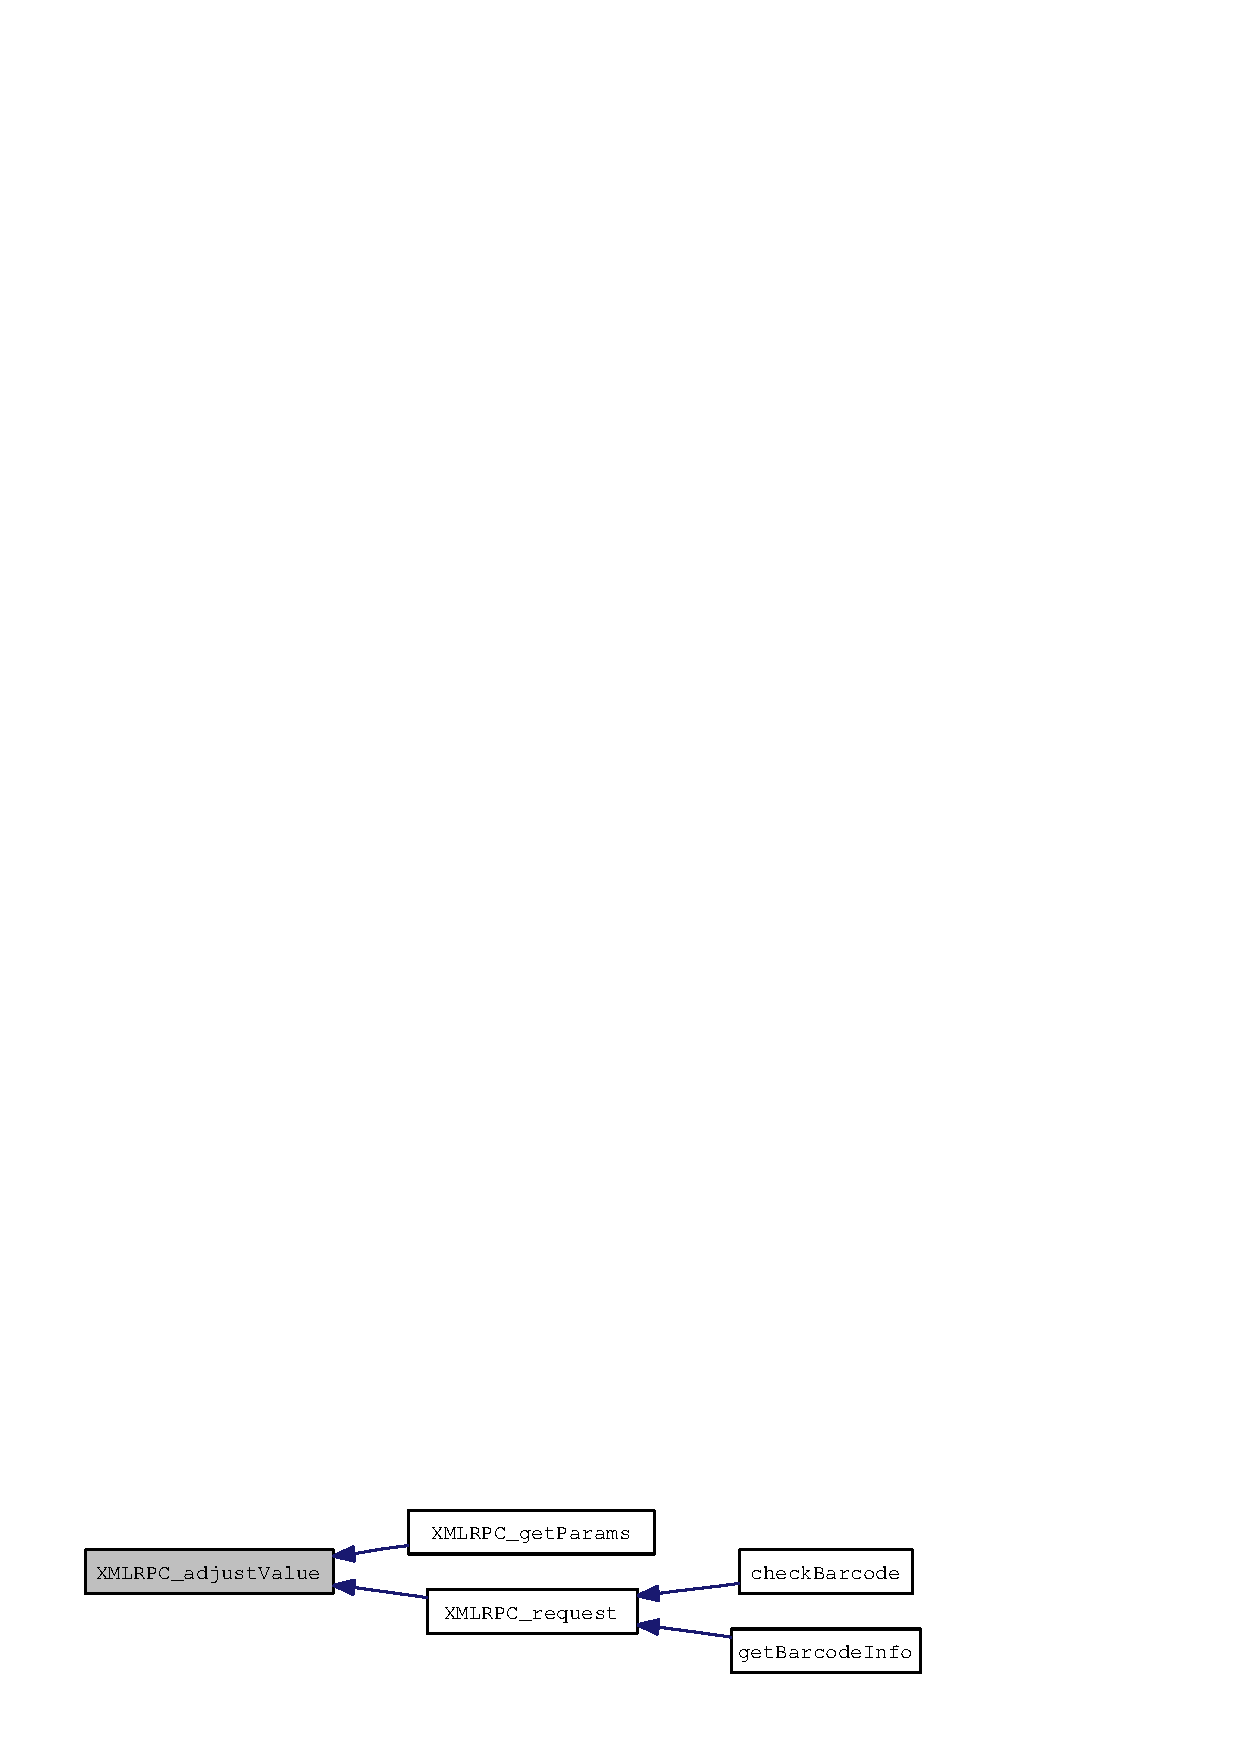
\includegraphics[width=223pt]{xmlrpc_8inc_d936fe41ae9c3e0b90bd72ffe82a2969_icgraph}
\end{center}
\end{figure}
\hypertarget{xmlrpc_8inc_1d9c2ef61c9f1fd2723d06d1364ef845}{
\index{xmlrpc.inc@{xmlrpc.inc}!XMLRPC_convert_iso8601_to_timestamp@{XMLRPC\_\-convert\_\-iso8601\_\-to\_\-timestamp}}
\index{XMLRPC_convert_iso8601_to_timestamp@{XMLRPC\_\-convert\_\-iso8601\_\-to\_\-timestamp}!xmlrpc.inc@{xmlrpc.inc}}
\subsubsection{\setlength{\rightskip}{0pt plus 5cm}XMLRPC\_\-convert\_\-iso8601\_\-to\_\-timestamp (\$ {\em iso8601})}}
\label{xmlrpc_8inc_1d9c2ef61c9f1fd2723d06d1364ef845}




Definition at line 461 of file xmlrpc.inc.

\begin{Code}\begin{verbatim}461                                                       {
462   return strtotime($iso8601);
463 }
\end{verbatim}
\end{Code}


\hypertarget{xmlrpc_8inc_4485d809c5d598949d9cfaca42bddf37}{
\index{xmlrpc.inc@{xmlrpc.inc}!XMLRPC_convert_timestamp_to_iso8601@{XMLRPC\_\-convert\_\-timestamp\_\-to\_\-iso8601}}
\index{XMLRPC_convert_timestamp_to_iso8601@{XMLRPC\_\-convert\_\-timestamp\_\-to\_\-iso8601}!xmlrpc.inc@{xmlrpc.inc}}
\subsubsection{\setlength{\rightskip}{0pt plus 5cm}XMLRPC\_\-convert\_\-timestamp\_\-to\_\-iso8601 (\$ {\em timestamp})}}
\label{xmlrpc_8inc_4485d809c5d598949d9cfaca42bddf37}




Definition at line 455 of file xmlrpc.inc.

\begin{Code}\begin{verbatim}455                                                         {
456   #takes a unix timestamp and converts it to iso8601 required by XMLRPC
457   #an example iso8601 datetime is "20010822T03:14:33"
458   return date("Ymd\TH:i:s", $timestamp);
459 }
\end{verbatim}
\end{Code}


\hypertarget{xmlrpc_8inc_e2d2e97a8c1c560f5e96d58d60a02874}{
\index{xmlrpc.inc@{xmlrpc.inc}!XMLRPC_debug@{XMLRPC\_\-debug}}
\index{XMLRPC_debug@{XMLRPC\_\-debug}!xmlrpc.inc@{xmlrpc.inc}}
\subsubsection{\setlength{\rightskip}{0pt plus 5cm}XMLRPC\_\-debug (\$ {\em function\_\-name}, \$ {\em debug\_\-message})}}
\label{xmlrpc_8inc_e2d2e97a8c1c560f5e96d58d60a02874}




Definition at line 469 of file xmlrpc.inc.

Referenced by XMLRPC\_\-error(), XMLRPC\_\-parse(), XMLRPC\_\-request(), and XMLRPC\_\-response().

\begin{Code}\begin{verbatim}469                                                      {
470   $GLOBALS['XMLRPC_DEBUG_INFO'][] = array($function_name, $debug_message);
471 }
\end{verbatim}
\end{Code}




Here is the caller graph for this function:\nopagebreak
\begin{figure}[H]
\begin{center}
\leavevmode
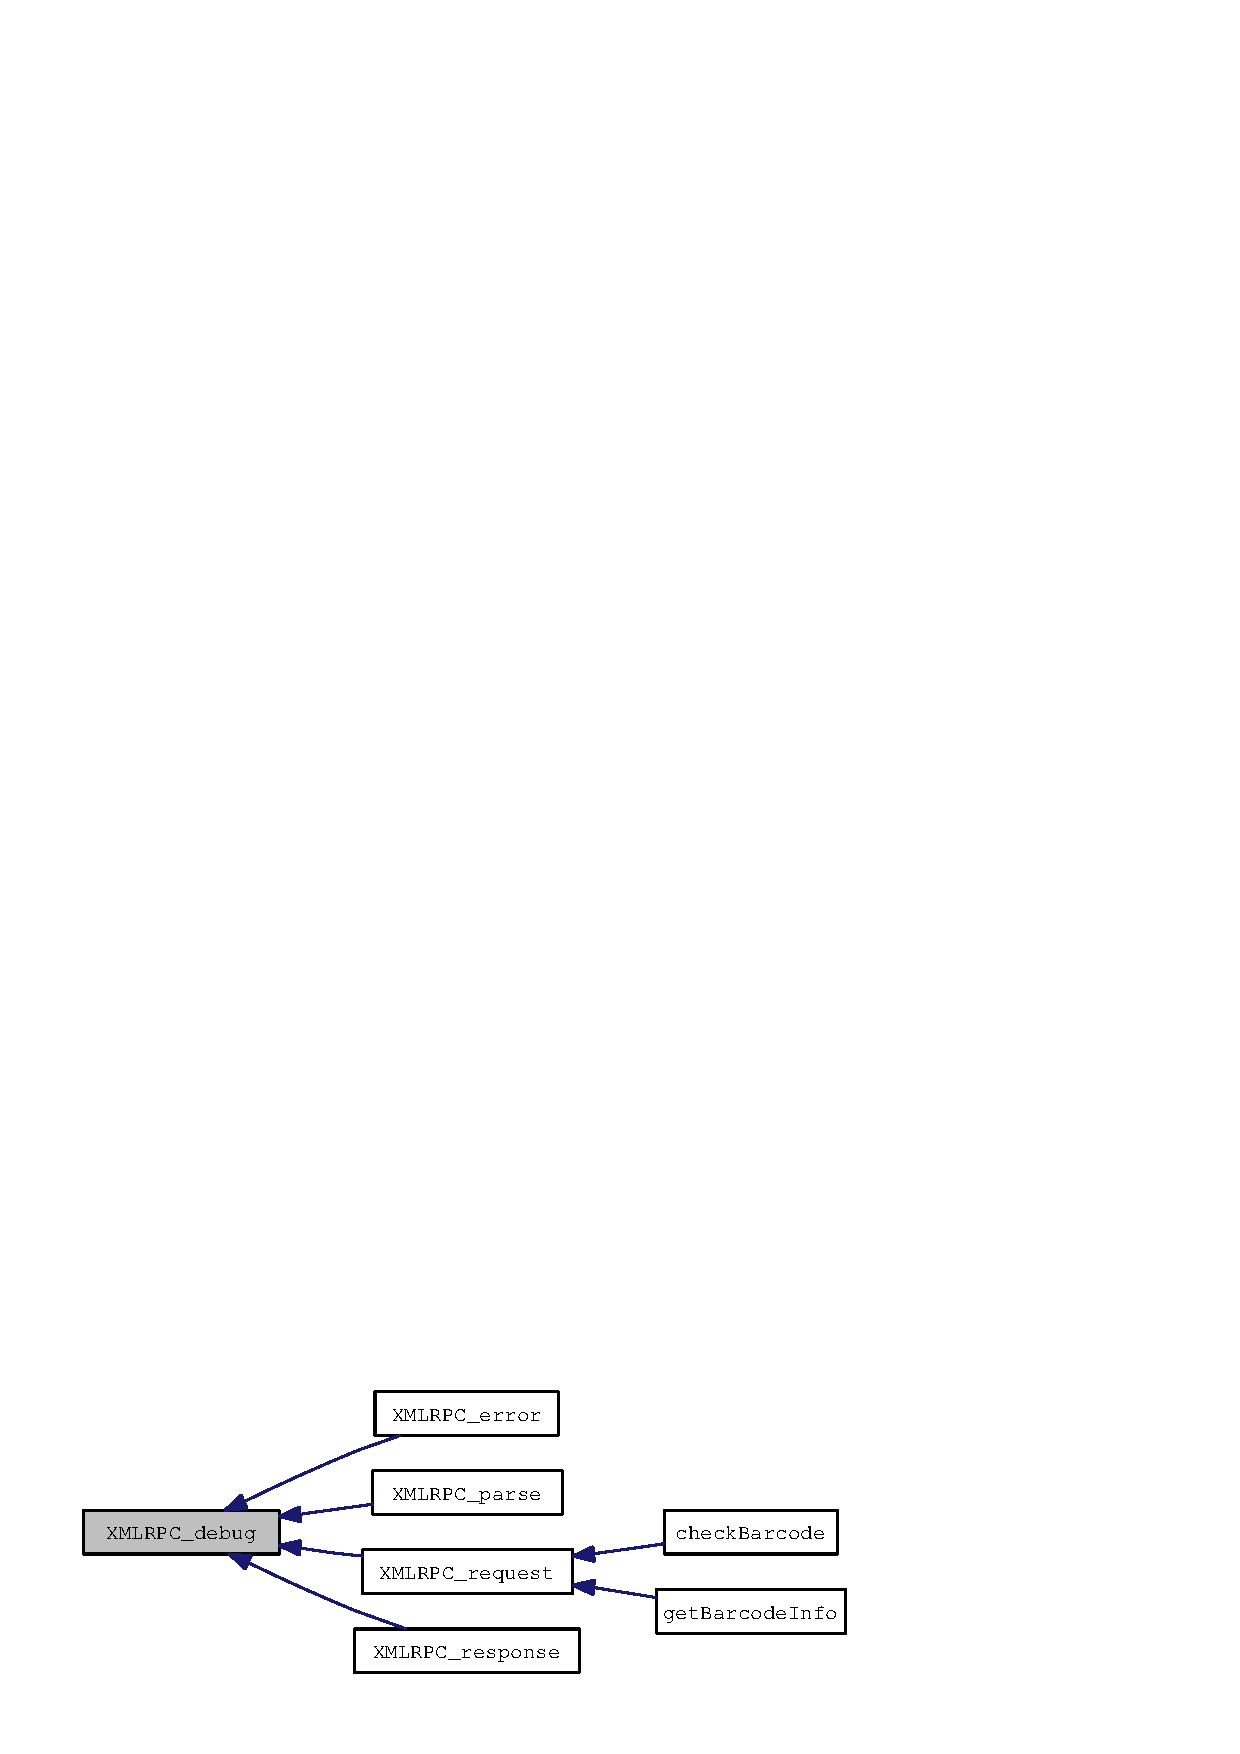
\includegraphics[width=205pt]{xmlrpc_8inc_e2d2e97a8c1c560f5e96d58d60a02874_icgraph}
\end{center}
\end{figure}
\hypertarget{xmlrpc_8inc_8467f85edd385ddf2506b1bd5065a6d7}{
\index{xmlrpc.inc@{xmlrpc.inc}!XMLRPC_debug_print@{XMLRPC\_\-debug\_\-print}}
\index{XMLRPC_debug_print@{XMLRPC\_\-debug\_\-print}!xmlrpc.inc@{xmlrpc.inc}}
\subsubsection{\setlength{\rightskip}{0pt plus 5cm}XMLRPC\_\-debug\_\-print ()}}
\label{xmlrpc_8inc_8467f85edd385ddf2506b1bd5065a6d7}




Definition at line 473 of file xmlrpc.inc.

References \$debug.

\begin{Code}\begin{verbatim}473                              {
474   if($GLOBALS['XMLRPC_DEBUG_INFO']){
475     echo "<table border=\"1\" width=\"100%\">\n";
476     foreach($GLOBALS['XMLRPC_DEBUG_INFO'] as $debug){
477       echo "<tr><th style=\"vertical-align: top\">$debug[0]</th><td>$debug[1]</td></tr>\n";
478     }
479     echo "</table>\n";
480     unset($GLOBALS['XMLRPC_DEBUG_INFO']);
481   }else{
482     echo "<p>No debugging information available yet.</p>";
483   }
484 }
\end{verbatim}
\end{Code}


\hypertarget{xmlrpc_8inc_0cdc54b1376ccbbe412175c9819a95ac}{
\index{xmlrpc.inc@{xmlrpc.inc}!XMLRPC_error@{XMLRPC\_\-error}}
\index{XMLRPC_error@{XMLRPC\_\-error}!xmlrpc.inc@{xmlrpc.inc}}
\subsubsection{\setlength{\rightskip}{0pt plus 5cm}XMLRPC\_\-error (\$ {\em faultCode}, \$ {\em faultString}, \$ {\em server} = {\tt NULL})}}
\label{xmlrpc_8inc_0cdc54b1376ccbbe412175c9819a95ac}




Definition at line 432 of file xmlrpc.inc.

References XML\_\-serialize(), XMLRPC\_\-debug(), and XMLRPC\_\-show().

\begin{Code}\begin{verbatim}432                                                                {
433   $array["methodResponse"]["fault"]["value"]["struct"]["member"] = array();
434   $temp = &$array["methodResponse"]["fault"]["value"]["struct"]["member"];
435   $temp[0]["name"] = "faultCode";
436   $temp[0]["value"]["int"] = $faultCode;
437   $temp[1]["name"] = "faultString";
438   $temp[1]["value"]["string"] = $faultString;
439 
440   $return = XML_serialize($array);
441 
442   header("Connection: close");
443   header("Content-Length: " . strlen($return));
444   header("Content-Type: text/xml");
445   header("Date: " . date("r"));
446   if($server){
447     header("Server: $server");
448   }
449   if(defined('XMLRPC_DEBUG') and XMLRPC_DEBUG){
450     XMLRPC_debug('XMLRPC_error', "<p>Sent the following error response:</p>\n\n" . XMLRPC_show($return, 'print_r', true));
451   }
452   echo $return;
453 }
\end{verbatim}
\end{Code}




Here is the call graph for this function:\nopagebreak
\begin{figure}[H]
\begin{center}
\leavevmode
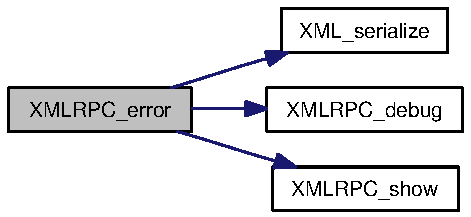
\includegraphics[width=131pt]{xmlrpc_8inc_0cdc54b1376ccbbe412175c9819a95ac_cgraph}
\end{center}
\end{figure}
\hypertarget{xmlrpc_8inc_70efa062e92a380196ed8053850c0906}{
\index{xmlrpc.inc@{xmlrpc.inc}!XMLRPC_getMethodName@{XMLRPC\_\-getMethodName}}
\index{XMLRPC_getMethodName@{XMLRPC\_\-getMethodName}!xmlrpc.inc@{xmlrpc.inc}}
\subsubsection{\setlength{\rightskip}{0pt plus 5cm}XMLRPC\_\-getMethodName (\$ {\em methodCall})}}
\label{xmlrpc_8inc_70efa062e92a380196ed8053850c0906}




Definition at line 331 of file xmlrpc.inc.

\begin{Code}\begin{verbatim}331                                           {
332   #returns the method name
333   return $methodCall['methodCall']['methodName'];
334 }
\end{verbatim}
\end{Code}


\hypertarget{xmlrpc_8inc_ce4ea8e1274ca2ee3f51ec5a724f00f3}{
\index{xmlrpc.inc@{xmlrpc.inc}!XMLRPC_getParams@{XMLRPC\_\-getParams}}
\index{XMLRPC_getParams@{XMLRPC\_\-getParams}!xmlrpc.inc@{xmlrpc.inc}}
\subsubsection{\setlength{\rightskip}{0pt plus 5cm}XMLRPC\_\-getParams (\$ {\em request})}}
\label{xmlrpc_8inc_ce4ea8e1274ca2ee3f51ec5a724f00f3}




Definition at line 310 of file xmlrpc.inc.

References XMLRPC\_\-adjustValue().

\begin{Code}\begin{verbatim}310                                    {
311   if(!is_array($request['methodCall']['params'])){
312     #If there are no parameters, return an empty array
313     return array();
314   }else{
315     #echo "Getting rid of methodCall -> params -> param<br>\n";
316     $temp = &$request['methodCall']['params']['param'];
317     if(is_array($temp) and array_key_exists(0, $temp)){
318       $count = count($temp);
319       for($n = 0; $n < $count; $n++){
320         #echo "Serializing parameter $n<br>";
321         $temp2[$n] = &XMLRPC_adjustValue(&$temp[$n]['value']);
322       }
323     }else{
324       $temp2[0] = &XMLRPC_adjustValue($temp['value']);
325     }
326     $temp = &$temp2;
327     return $temp;
328   }
329 }
\end{verbatim}
\end{Code}




Here is the call graph for this function:\nopagebreak
\begin{figure}[H]
\begin{center}
\leavevmode
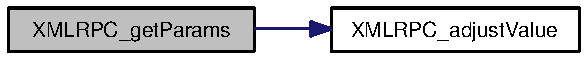
\includegraphics[width=159pt]{xmlrpc_8inc_ce4ea8e1274ca2ee3f51ec5a724f00f3_cgraph}
\end{center}
\end{figure}
\hypertarget{xmlrpc_8inc_708b2136ca600664d2207a511b3cf3f8}{
\index{xmlrpc.inc@{xmlrpc.inc}!XMLRPC_parse@{XMLRPC\_\-parse}}
\index{XMLRPC_parse@{XMLRPC\_\-parse}!xmlrpc.inc@{xmlrpc.inc}}
\subsubsection{\setlength{\rightskip}{0pt plus 5cm}\& XMLRPC\_\-parse (\&\$ {\em request})}}
\label{xmlrpc_8inc_708b2136ca600664d2207a511b3cf3f8}




Definition at line 166 of file xmlrpc.inc.

References XML\_\-unserialize(), XMLRPC\_\-debug(), and XMLRPC\_\-show().

\begin{Code}\begin{verbatim}166                                   {
167   if(defined('XMLRPC_DEBUG') and XMLRPC_DEBUG){
168     XMLRPC_debug('XMLRPC_parse', "<p>Received the following raw request:</p>" . XMLRPC_show($request, 'print_r', true));
169   }
170   $data = &XML_unserialize(&$request);
171   if(defined('XMLRPC_DEBUG') and XMLRPC_DEBUG){
172     XMLRPC_debug('XMLRPC_parse', "<p>Returning the following parsed request:</p>" . XMLRPC_show($data, 'print_r', true));
173   }
174   return $data;
175 }
\end{verbatim}
\end{Code}




Here is the call graph for this function:\nopagebreak
\begin{figure}[H]
\begin{center}
\leavevmode
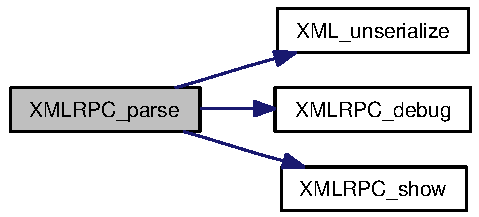
\includegraphics[width=133pt]{xmlrpc_8inc_708b2136ca600664d2207a511b3cf3f8_cgraph}
\end{center}
\end{figure}
\hypertarget{xmlrpc_8inc_c13be54b26e0803d8745e4f019dcfd8a}{
\index{xmlrpc.inc@{xmlrpc.inc}!XMLRPC_prepare@{XMLRPC\_\-prepare}}
\index{XMLRPC_prepare@{XMLRPC\_\-prepare}!xmlrpc.inc@{xmlrpc.inc}}
\subsubsection{\setlength{\rightskip}{0pt plus 5cm}\& XMLRPC\_\-prepare (\$ {\em data}, \$ {\em type} = {\tt NULL})}}
\label{xmlrpc_8inc_c13be54b26e0803d8745e4f019dcfd8a}




Definition at line 177 of file xmlrpc.inc.

References count\_\-numeric\_\-items().

Referenced by checkBarcode(), and getBarcodeInfo().

\begin{Code}\begin{verbatim}177                                               {
178   if(is_array($data)){
179     $num_elements = count($data);
180     if((array_key_exists(0, $data) or !$num_elements) and $type != 'struct'){ #it's an array
181       if(!$num_elements){ #if the array is empty
182         $returnvalue =  array('array' => array('data' => NULL));
183       }else{
184         $returnvalue['array']['data']['value'] = array();
185         $temp = &$returnvalue['array']['data']['value'];
186         $count = count_numeric_items($data);
187         for($n=0; $n<$count; $n++){
188           $type = NULL;
189           if(array_key_exists("$n type", $data)){
190             $type = $data["$n type"];
191           }
192           $temp[$n] = XMLRPC_prepare(&$data[$n], $type);
193         }
194       }
195     }else{ #it's a struct
196       if(!$num_elements){ #if the struct is empty
197         $returnvalue = array('struct' => NULL);
198       }else{
199         $returnvalue['struct']['member'] = array();
200         $temp = &$returnvalue['struct']['member'];
201         while(list($key, $value) = each($data)){
202           if(substr($key, -5) != ' type'){ #if it's not a type specifier
203             $type = NULL;
204             if(array_key_exists("$key type", $data)){
205               $type = $data["$key type"];
206             }
207             $temp[] = array('name' => $key, 'value' => XMLRPC_prepare(&$value, $type));
208           }
209         }
210       }
211     }
212   }else{ #it's a scalar
213     if(!$type){
214       if(is_int($data)){
215         $returnvalue['int'] = $data;
216         return $returnvalue;
217       }elseif(is_float($data)){
218         $returnvalue['double'] = $data;
219         return $returnvalue;
220       }elseif(is_bool($data)){
221         $returnvalue['boolean'] = ($data ? 1 : 0);
222         return $returnvalue;
223       }elseif(preg_match('/^\d{8}T\d{2}:\d{2}:\d{2}$/', $data, $matches)){ #it's a date
224         $returnvalue['dateTime.iso8601'] = $data;
225         return $returnvalue;
226       }elseif(is_string($data)){
227         $returnvalue['string'] = htmlspecialchars($data);
228         return $returnvalue;
229       }
230     }else{
231       $returnvalue[$type] = htmlspecialchars($data);
232     }
233   }
234   return $returnvalue;
235 }
\end{verbatim}
\end{Code}




Here is the call graph for this function:\nopagebreak
\begin{figure}[H]
\begin{center}
\leavevmode
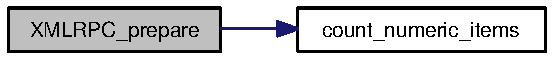
\includegraphics[width=151pt]{xmlrpc_8inc_c13be54b26e0803d8745e4f019dcfd8a_cgraph}
\end{center}
\end{figure}


Here is the caller graph for this function:\nopagebreak
\begin{figure}[H]
\begin{center}
\leavevmode
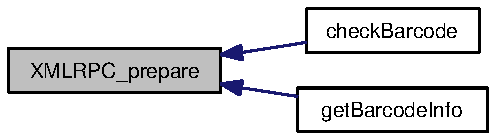
\includegraphics[width=137pt]{xmlrpc_8inc_c13be54b26e0803d8745e4f019dcfd8a_icgraph}
\end{center}
\end{figure}
\hypertarget{xmlrpc_8inc_3a98b6984b8ca01752d1aa9a267526a3}{
\index{xmlrpc.inc@{xmlrpc.inc}!XMLRPC_request@{XMLRPC\_\-request}}
\index{XMLRPC_request@{XMLRPC\_\-request}!xmlrpc.inc@{xmlrpc.inc}}
\subsubsection{\setlength{\rightskip}{0pt plus 5cm}XMLRPC\_\-request (\$ {\em site}, \$ {\em location}, \$ {\em methodName}, \$ {\em params} = {\tt NULL}, \$ {\em user\_\-agent} = {\tt NULL})}}
\label{xmlrpc_8inc_3a98b6984b8ca01752d1aa9a267526a3}




Definition at line 336 of file xmlrpc.inc.

References XML\_\-serialize(), XML\_\-unserialize(), XMLRPC\_\-adjustValue(), XMLRPC\_\-debug(), and XMLRPC\_\-show().

Referenced by checkBarcode(), and getBarcodeInfo().

\begin{Code}\begin{verbatim}336                                                                                           {
337   $site = explode(':', $site);
338   if(isset($site[1]) and is_numeric($site[1])){
339     $port = $site[1];
340   }else{
341     $port = 80;
342   }
343   $site = $site[0];
344 
345   $data["methodCall"]["methodName"] = $methodName;
346   $param_count = count($params);
347   if(!$param_count){
348     $data["methodCall"]["params"] = NULL;
349   }else{
350     for($n = 0; $n<$param_count; $n++){
351       $data["methodCall"]["params"]["param"][$n]["value"] = $params[$n];
352     }
353   }
354   $data = XML_serialize($data);
355 
356   if(defined('XMLRPC_DEBUG') and XMLRPC_DEBUG){
357     XMLRPC_debug('XMLRPC_request', "<p>Received the following parameter list to send:</p>" . XMLRPC_show($params, 'print_r', true));
358   }
359   $conn = fsockopen ($site, $port); #open the connection
360   if(!$conn){ #if the connection was not opened successfully
361     if(defined('XMLRPC_DEBUG') and XMLRPC_DEBUG){
362       XMLRPC_debug('XMLRPC_request', "<p>Connection failed: Couldn't make the connection to $site.</p>");
363     }
364     return array(false, array('faultCode'=>10532, 'faultString'=>"Connection failed: Couldn't make the connection to $site."));
365   }else{
366     $headers =
367       "POST $location HTTP/1.0\r\n" .
368       "Host: $site\r\n" .
369       "Connection: close\r\n" .
370       ($user_agent ? "User-Agent: $user_agent\r\n" : '') .
371       "Content-Type: text/xml\r\n" .
372       "Content-Length: " . strlen($data) . "\r\n\r\n";
373 
374     fputs($conn, "$headers");
375     fputs($conn, $data);
376 
377     if(defined('XMLRPC_DEBUG') and XMLRPC_DEBUG){
378       XMLRPC_debug('XMLRPC_request', "<p>Sent the following request:</p>\n\n" . XMLRPC_show($headers . $data, 'print_r', true));
379     }
380 
381     #socket_set_blocking ($conn, false);
382     $response = "";
383     while(!feof($conn)){
384       $response .= fgets($conn, 1024);
385     }
386     fclose($conn);
387 
388     #strip headers off of response
389     $data = XML_unserialize(substr($response, strpos($response, "\r\n\r\n")+4));
390 
391     if(defined('XMLRPC_DEBUG') and XMLRPC_DEBUG){
392       XMLRPC_debug('XMLRPC_request', "<p>Received the following response:</p>\n\n" . XMLRPC_show($response, 'print_r', true) . "<p>Which was serialized into the following data:</p>\n\n" . XMLRPC_show($data, 'print_r', true));
393     }
394     if(isset($data['methodResponse']['fault'])){
395       $return =  array(false, XMLRPC_adjustValue(&$data['methodResponse']['fault']['value']));
396       if(defined('XMLRPC_DEBUG') and XMLRPC_DEBUG){
397         XMLRPC_debug('XMLRPC_request', "<p>Returning:</p>\n\n" . XMLRPC_show($return, 'var_dump', true));
398       }
399       return $return;
400     }else{
401       $return = array(true, XMLRPC_adjustValue(&$data['methodResponse']['params']['param']['value']));
402       if(defined('XMLRPC_DEBUG') and XMLRPC_DEBUG){
403         XMLRPC_debug('XMLRPC_request', "<p>Returning:</p>\n\n" . XMLRPC_show($return, 'var_dump', true));
404       }
405       return $return;
406     }
407   }
408 }
\end{verbatim}
\end{Code}




Here is the call graph for this function:\nopagebreak
\begin{figure}[H]
\begin{center}
\leavevmode
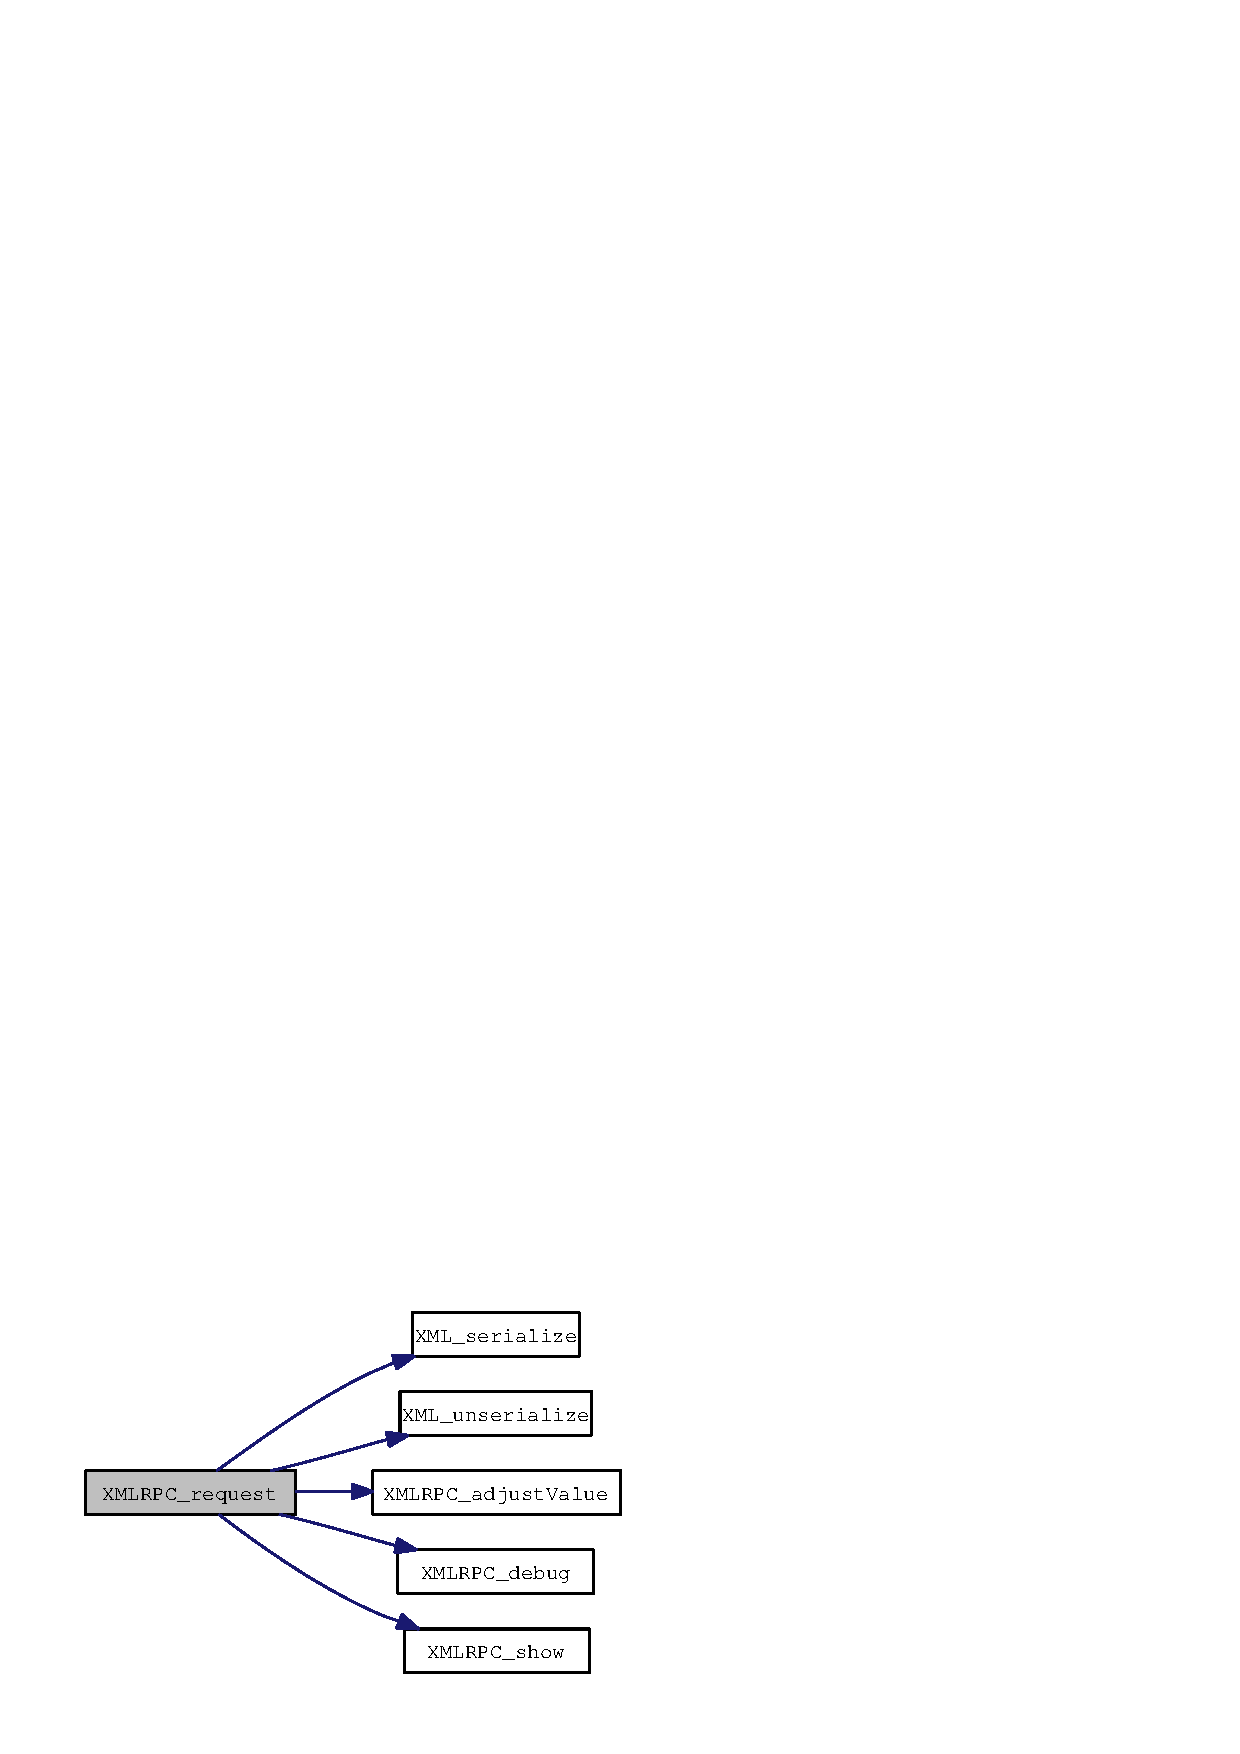
\includegraphics[width=151pt]{xmlrpc_8inc_3a98b6984b8ca01752d1aa9a267526a3_cgraph}
\end{center}
\end{figure}


Here is the caller graph for this function:\nopagebreak
\begin{figure}[H]
\begin{center}
\leavevmode
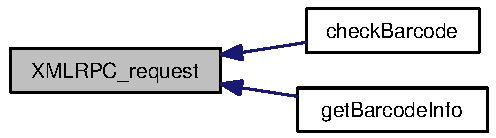
\includegraphics[width=137pt]{xmlrpc_8inc_3a98b6984b8ca01752d1aa9a267526a3_icgraph}
\end{center}
\end{figure}
\hypertarget{xmlrpc_8inc_c736d378caaccdd0726ea1080d1f526f}{
\index{xmlrpc.inc@{xmlrpc.inc}!XMLRPC_response@{XMLRPC\_\-response}}
\index{XMLRPC_response@{XMLRPC\_\-response}!xmlrpc.inc@{xmlrpc.inc}}
\subsubsection{\setlength{\rightskip}{0pt plus 5cm}XMLRPC\_\-response (\$ {\em return\_\-value}, \$ {\em server} = {\tt NULL})}}
\label{xmlrpc_8inc_c736d378caaccdd0726ea1080d1f526f}




Definition at line 410 of file xmlrpc.inc.

References XML\_\-serialize(), XMLRPC\_\-debug(), and XMLRPC\_\-show().

\begin{Code}\begin{verbatim}410                                                        {
411   $data["methodResponse"]["params"]["param"]["value"] = &$return_value;
412   $return = XML_serialize(&$data);
413 
414   if(defined('XMLRPC_DEBUG') and XMLRPC_DEBUG){
415     XMLRPC_debug('XMLRPC_response', "<p>Received the following data to return:</p>\n\n" . XMLRPC_show($return_value, 'print_r', true));
416   }
417 
418   header("Connection: close");
419   header("Content-Length: " . strlen($return));
420   header("Content-Type: text/xml");
421   header("Date: " . date("r"));
422   if($server){
423     header("Server: $server");
424   }
425 
426   if(defined('XMLRPC_DEBUG') and XMLRPC_DEBUG){
427     XMLRPC_debug('XMLRPC_response', "<p>Sent the following response:</p>\n\n" . XMLRPC_show($return, 'print_r', true));
428   }
429   echo $return;
430 }
\end{verbatim}
\end{Code}




Here is the call graph for this function:\nopagebreak
\begin{figure}[H]
\begin{center}
\leavevmode
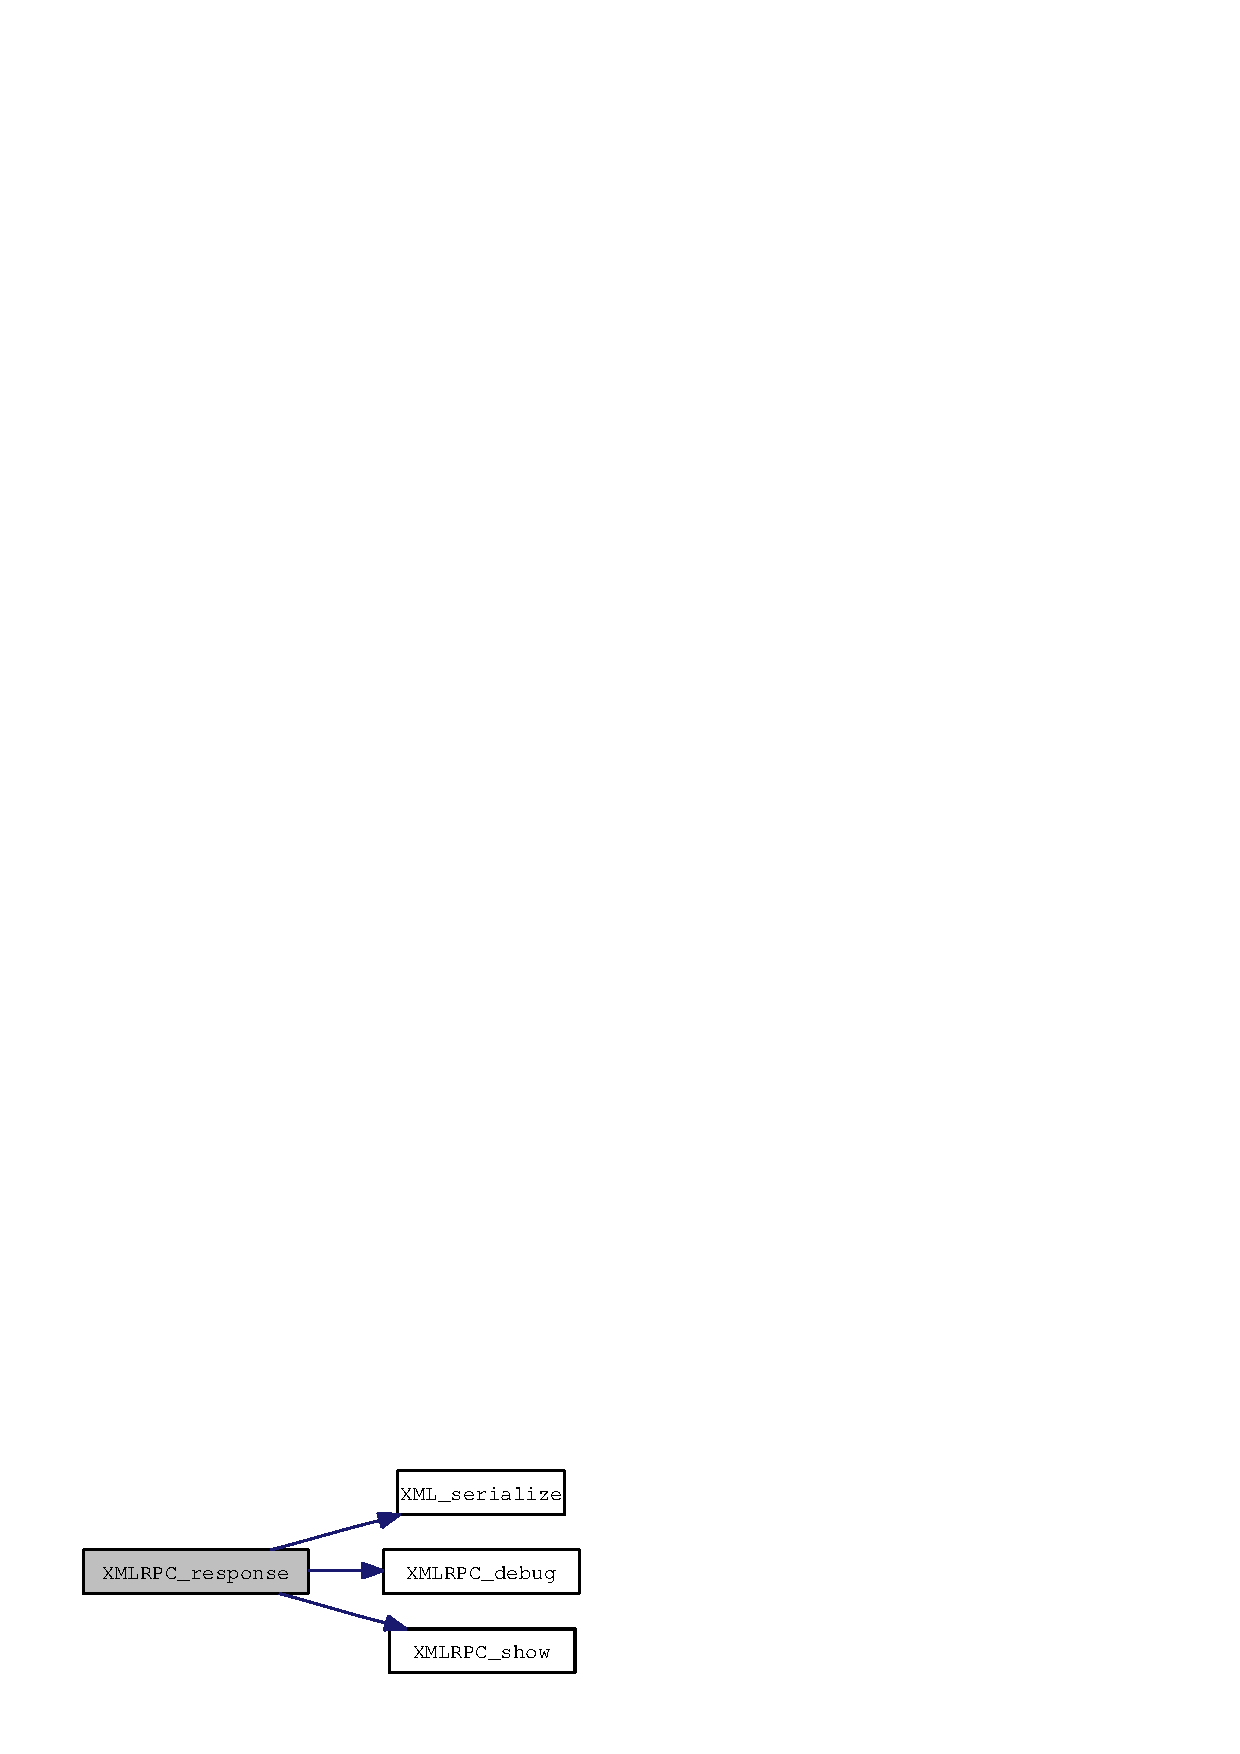
\includegraphics[width=141pt]{xmlrpc_8inc_c736d378caaccdd0726ea1080d1f526f_cgraph}
\end{center}
\end{figure}
\hypertarget{xmlrpc_8inc_1f60d2672bcb35f5ff908f64931f8d48}{
\index{xmlrpc.inc@{xmlrpc.inc}!XMLRPC_show@{XMLRPC\_\-show}}
\index{XMLRPC_show@{XMLRPC\_\-show}!xmlrpc.inc@{xmlrpc.inc}}
\subsubsection{\setlength{\rightskip}{0pt plus 5cm}XMLRPC\_\-show (\$ {\em data}, \$ {\em func} = {\tt \char`\"{}print\_\-r\char`\"{}}, \$ {\em return\_\-str} = {\tt false})}}
\label{xmlrpc_8inc_1f60d2672bcb35f5ff908f64931f8d48}




Definition at line 486 of file xmlrpc.inc.

Referenced by XMLRPC\_\-error(), XMLRPC\_\-parse(), XMLRPC\_\-request(), and XMLRPC\_\-response().

\begin{Code}\begin{verbatim}486                                                                    {
487   ob_start();
488   $func($data);
489   $output = ob_get_contents();
490   ob_end_clean();
491   if($return_str){
492     return "<pre>" . htmlspecialchars($output) . "</pre>\n";
493   }else{
494     echo "<pre>", htmlspecialchars($output), "</pre>\n";
495   }
496 }
\end{verbatim}
\end{Code}




Here is the caller graph for this function:\nopagebreak
\begin{figure}[H]
\begin{center}
\leavevmode
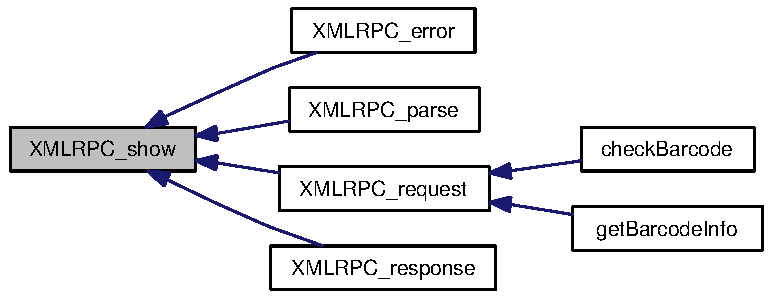
\includegraphics[width=203pt]{xmlrpc_8inc_1f60d2672bcb35f5ff908f64931f8d48_icgraph}
\end{center}
\end{figure}
